\documentclass[border=3pt]{standalone}
% Preâmbulo compartilhado pelos diagramas TikZ da aula 8 de IHR (Métodos de Pesquisa)
\usepackage[T1]{fontenc}
\usepackage[utf8]{inputenc}
\usepackage{lmodern}
\usepackage{amsmath}
\usepackage{xcolor}
\usepackage{tikz}
\usetikzlibrary{arrows.meta,angles,quotes,decorations.pathmorphing,decorations.pathreplacing,calc,
                positioning,shapes.geometric,shapes.misc,backgrounds,fit,
                math}

% Paleta (mesma dos SVGs originais)
% Paleta da disciplina de IHR: acento azul (#1A6FB5), cor de destaque do tema.
% (o nome "dblue" é mantido para não alterar todos os diagramas)
\definecolor{dblue}{HTML}{1A6FB5}
\definecolor{dorange}{HTML}{B3541E}
\definecolor{dgreen}{HTML}{4A7C59}
\definecolor{dred}{HTML}{9C4B4B}
\definecolor{dcream}{HTML}{F4F1EA}
\definecolor{dshade}{HTML}{DDD7C9}

% Função gaussiana (não normalizada por padrão de escala visual)
\pgfmathdeclarefunction{gauss}{3}{%
  \pgfmathparse{1/(#3*sqrt(2*pi))*exp(-((#1-#2)^2)/(2*#3^2))}%
}

% Estilos comuns (prefixo d... para não colidir com chaves internas do pgf)
\tikzset{
  >={Stealth[length=2mm]},
  dguide/.style={gray!55, dashed, line width=0.4pt},
  daxis/.style={gray!60, line width=0.7pt, ->},
  dbody/.style={fill=black!3, draw=black!80, line width=1pt},
  dacc/.style={draw=dblue, line width=1pt},
  dlbl/.style={black!55, font=\small},
  dsub/.style={black!45, font=\footnotesize},
  dstate/.style={circle, draw=black!80, fill=dcream, line width=1pt,
                 minimum size=17mm, font=\large, inner sep=1pt},
  dobs/.style={circle, draw=black!80, fill=dshade, line width=1pt,
               minimum size=14mm, font=\large, inner sep=1pt},
  dbox/.style={rounded corners=2pt, draw=black!80, fill=dcream, line width=1pt,
               align=center, inner sep=6pt},
  dop/.style={circle, draw=black!80, fill=white, line width=1pt,
              minimum size=6mm, inner sep=0pt, font=\small},
  dtrans/.style={->, dblue, line width=1pt},
  dmeas/.style={->, dorange, line width=1pt},
  dcurve/.style={line width=1pt, dblue},
  dcurveb/.style={line width=1.4pt, dorange},
}

\begin{document}
\hyphenpenalty=10000 \exhyphenpenalty=10000 \tolerance=9999 \emergencystretch=3em
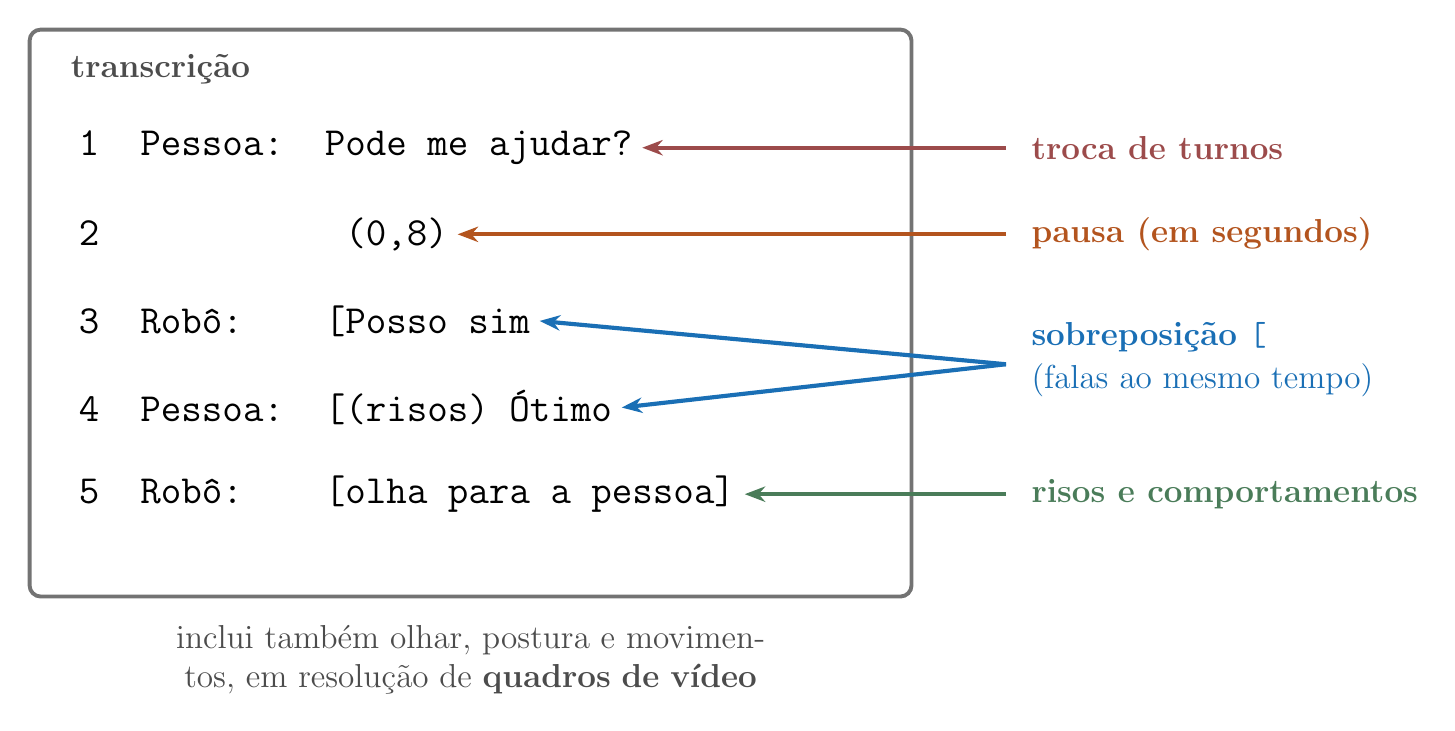
\begin{tikzpicture}[x=1cm,y=1cm]
  \draw[dbox, draw=black!55, fill=white, line width=1.4pt, rounded corners=4pt] (0.2,0.4) rectangle (11.4,7.6);
  \node[font=\large\bfseries, black!70, anchor=west] at (0.6,7.1) {transcrição};
  \node[font=\Large\ttfamily, anchor=west] (l1) at (0.7,6.1) {1\ \ Pessoa:\ \ Pode me ajudar?};
  \node[font=\Large\ttfamily, anchor=west] (l2) at (0.7,5.0) {2\ \ \ \ \ \ \ \ \ \ \ \ (0,8)};
  \node[font=\Large\ttfamily, anchor=west] (l3) at (0.7,3.9) {3\ \ Robô:\ \ \ \ [Posso sim};
  \node[font=\Large\ttfamily, anchor=west] (l4) at (0.7,2.8) {4\ \ Pessoa:\ \ [(risos) Ótimo};
  \node[font=\Large\ttfamily, anchor=west] (l5) at (0.7,1.7) {5\ \ Robô:\ \ \ \ {[}olha para a pessoa{]}};
  \draw[dred, line width=1.5pt, -{Stealth[length=2.6mm]}] (12.6,6.1) -- (l1.east);
  \node[font=\large\bfseries, dred, anchor=west] at (12.8,6.1) {troca de turnos};
  \draw[dorange, line width=1.5pt, -{Stealth[length=2.6mm]}] (12.6,5.0) -- (l2.east);
  \node[font=\large\bfseries, dorange, anchor=west] at (12.8,5.0) {pausa (em segundos)};
  \draw[dblue, line width=1.5pt, -{Stealth[length=2.6mm]}] (12.6,3.35) -- (l3.east);
  \draw[dblue, line width=1.5pt, -{Stealth[length=2.6mm]}] (12.6,3.35) -- (l4.east);
  \node[font=\large\bfseries, dblue, anchor=west] at (12.8,3.7) {sobreposição \texttt{[}};
  \node[font=\large, dblue, anchor=west] at (12.8,3.15) {(falas ao mesmo tempo)};
  \draw[dgreen, line width=1.5pt, -{Stealth[length=2.6mm]}] (12.6,1.7) -- (l5.east);
  \node[font=\large\bfseries, dgreen, anchor=west] at (12.8,1.7) {risos e comportamentos};
  \node[font=\large, black!70, text width=11cm, align=center] at (5.8,-0.4) {inclui também olhar, postura e movimentos, em resolução de \textbf{quadros de vídeo}};
\end{tikzpicture}
\end{document}
